\documentclass{article}
\usepackage[a4paper, total={6in, 8in}]{geometry}
\usepackage{graphicx}
\usepackage{hyperref}
\renewcommand*{\thesection}{\Roman{section}}
\begin{document}

\date{04/2024}

\title{\Large \bf Report: communcation jitter analysis, periodic peaks}

\author{Davide Rovelli, Michele Dalle Rive}
\maketitle

\section{Objective}
We analyse the latency disitribution in the communication between 2 bare-metal 
nodes in a datacenter. The objective of our experiments is to make packet 
processing latency of Linux-based hosts with modern NICs as \textit{deterministic}
as possible. This consists in reducing communication jitter to a minimum, where
$jitter = \max(latency) - \min(latency)$.

Contrarily to usual low tail-latency experiments/systems which aim to reduce the
common-case latency up to some percentile (e.g.$99.5\%, 99.9\%$) we want to minimise 
the $100\%$ latency, even at the cost of (non-substantially) increasing the 
common-case. 

\section{Methodology}

\subsection{Benchmark}
\label{sec:benchmark}
We run ping-pong tests across 2 hosts \textbf{A} and \textbf{B} by sending packets
at a fixed sending rate. Each packet carries a packet ID and 4 timestamps:

\begin{itemize}
  \itemsep=-0.8mm
  \item $ts_1$: timestamp just before sending the PING message in host \textbf{A}
  \item $ts_2$: timestamp as soon as the process in host \textbf{B} receives the
  PING packet.
  \item $ts_3$: timestamp just before sending the PONG message in host \textbf{B}
  \item $ts_4$: timestamp as soon as the process in host \textbf{A} receives the
  PONG packet.
\end{itemize}

We then calculate the difference between timestamps of successive packets
to get the variations in latency. For example, $ts_1(33) - ts_1(32)$ where 33 and
32 are the packet IDs, represents the time interval between the PING send timestamp
of packet 32 and the PING send timestamp of packet 33. If there's no jitter,
it should be equal to the sending rate. The difference between $ts_1(33) - ts_1(32)$
and the sending rate represents the relative jitter for that pair. 

\subsection{Hardware setup}
\paragraph{Cluster A} 2x CloudLab xl170 nodes

\begin{itemize}
  \itemsep=-0.8mm
  \item CPU:  Intel Xeon E5-2640 v4 at 2.40GHz, 10 cores, 64GB RAM
  \item OS/kernel: Ubuntu 22.04.4 LTS / 6.6.19-060619-generic x86\_64
  \item NIC/driver: Mellanox Connect-X 4 / mlx5 
\end{itemize}

% \paragraph{Cluster B} 2x internal cluster nodes: 

% \begin{itemize}
%   \itemsep=-0.8mm
%   \item CPU:  Intel Xeon E5-2680 v4 at 2.40GHz , 28 cores, 64GB RAM
%   \item OS/kernel: Ubuntu 22.04.4 LTS / 6.6.19-060619-generic x86\_64
%   \item NIC/driver: Mellanox Connect-X 4 / mlx5 
% \end{itemize}


Nodes are connected over ethernet, via a TOR switch with zero or minimal network load in order 
to only observe the endhost processing overhead.

\subsection{Software setup}
\label{sec:software}
We use different \textit{kernel bypass} methods in order to minimize the 
well-known overhead introduced by the classical network stack in Linux machines.
We test the following: 

\begin{itemize}
  \vspace{-0.8mm}
  \itemsep=-0.4mm
  \item RoCE, specifically double-sided SEND/RECV RDMA with the Unreliable Datagram (UD) 
  transport type
  \item eBPF XDP in two different modalities:
  \vspace{-1.8mm}
  \begin{itemize}
    \itemsep=-0.5mm
    \item XDP-offload: packet is handled by an eBPF XDP hook and executed as early
    as possible in the network stack 
    \item AF\_XDP: XDP socket type which handles TX and RX buffer management to 
    the application
  \end{itemize}
    \item Standard network stack over UDP    
\end{itemize}

\noindent
Packet size: \textit{1024 bytes}


\section{Analysis of periodic outliers}
Here we show some of the results which include interestingly periodic latency 
outliers, which we refer to as ``peaks''. We observe two types of periodic peaks 
of which we have not yet identified the root
cause. We refer to them as \textbf{$ts_1$-offset} and \textbf{$ts_2$-arrow}.

\autoref{fig:1} shows a typical benchmark containing a thick baseline around the 
sending rate ($996\mu s$), which means that most packets are subject to a minimal 
jitter apart from the the outlier types that we analyze below.

\paragraph*{$ts_1$-offset} The top-left plot in \autoref{fig:1}, representing the difference
between 2 successive send events of the PING packet on host A, shows 
\textbf{$ts_1$-offset}:
a small number of outliers delayed from baseline by a similar offset in the 
y-axis ($\approx150\mu s$). Successive outliers evenly spaced, meaning there is a 
fixed number of packet (i.e. time interval) between them. 

\paragraph*{$ts_2$-arrow} The top-right plot in \autoref{fig:1}, representing 
the difference 
between 2 successive receive events of the PING packet on host B, shows 
\textbf{$ts_2$-arrow}: a 
series of outliers with decreasing amplitude. Every outlier on top of the 
baseline (delayed packet) is immediately followed by a symmetric point below the
baseline which shows that the successive packet was not delayed, hence the 
difference between its timestamp and the one of the previous delayed packet is
less than then sending rate. 
Successive outliers forming the arrow are evenly spaced, meaning there is a 
fixed number of packet (i.e. time interval) between them. 


\paragraph*{} Bottom left and bottom right plot show no periodic outliers, 
meaning that the PONG send and receive events do not seem to be subject to
periodic peaks in our experiments. \textbf{$ts_1$-offset} and 
\textbf{$ts_2$-arrow} have the following characteristics:

\begin{itemize}
  \item Independent from the software technology used, they manifiest with all 
  bypass techniques listed in \autoref{sec:software} as well as the normal 
  network stack. 
  \item Throughput dependent: changing the sending rate changes some 
  characteristics as we cover in the next section
  \item Partially reproducible: 2 runs with the same settings often leads to the same
  result but not always, especially \textbf{$ts_2$-arrow} seems to be the most
  variable. 
  \item 
\end{itemize}



\begin{figure}
  \centering
  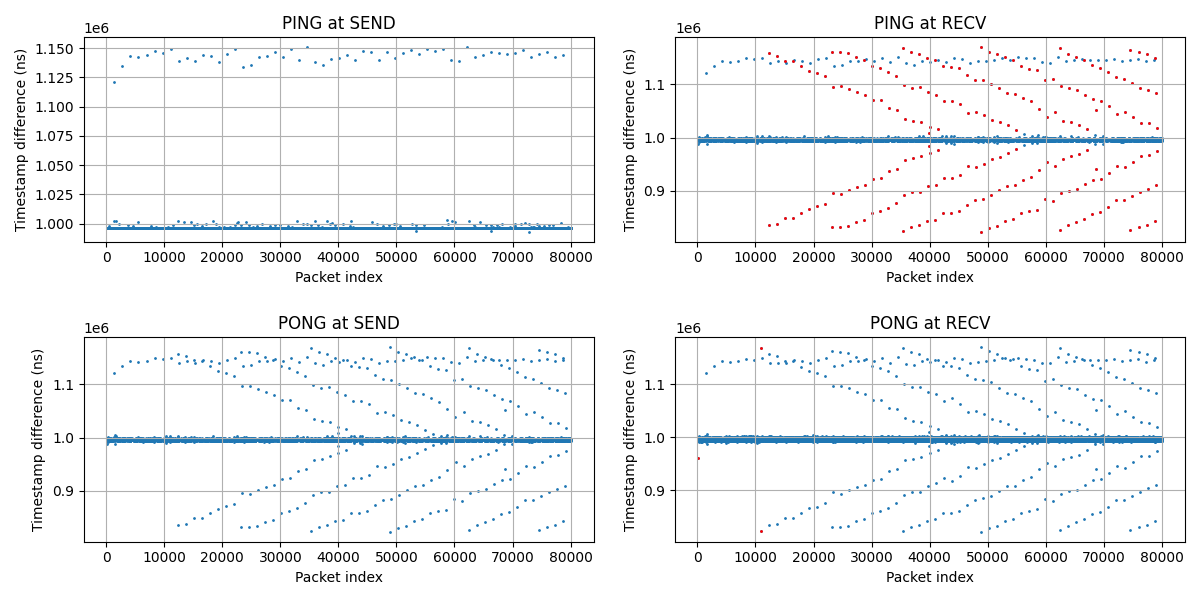
\includegraphics[width=\textwidth]{fig/xsk_80k_996us_powermax.png}
  \caption{Pingpong benchmark plot - sending interval $996\mu s$. Each dot corresponds 
  to a packet ID (x-axis) and the difference between its timestamp and the timestamp 
  of the packet with the previous ID (y-axis). The sending interval is fixed and 
  packets are sent in order. See \autoref{sec:benchmark} for a more detailed
  explanation of the benchmark}
  \label{fig:1}
\end{figure}


\end{document}